\documentclass{beamer}
\usepackage[utf8]{inputenc}
\usetheme{PaloAlto}
\usecolortheme{default}
\usepackage{tikz}
\usetikzlibrary{shapes,arrows,chains}

\title[Métodos de Segmentação Automática de Sinais de sEMG] % (optional, only for long titles)
{Métodos de Segmentação Automática de Sinais de Eletromiografia de Superfície}
\subtitle{para Classificação de Movimentos Utilizando RNA}
\author[Cunha] % (optional, for multiple authors)
{Vicente Cunha}
\institute[UFRGS] % (optional)
{
  Universidade Federal do Rio Grande do Sul
}
\date[dezembro de 2015] % (optional)
{Porto Alegre, dezembro de 2015}
\subject{Biomedical Science}

\begin{document}
	
	\frame{\titlepage}
	
	\begin{frame}
		\frametitle{Sumário}
		\tableofcontents[currentsection]
	\end{frame}
	
	\section[Introdução]{Introdução}
	
	\begin{frame}
		\frametitle{Eletromiografia}
		\framesubtitle{Principais aplicações}
		\begin{columns}[c]
			\column{.5\textwidth}
				\begin{figure}
					Diagnóstico de desordens neuromusculares
					\begin{center}
						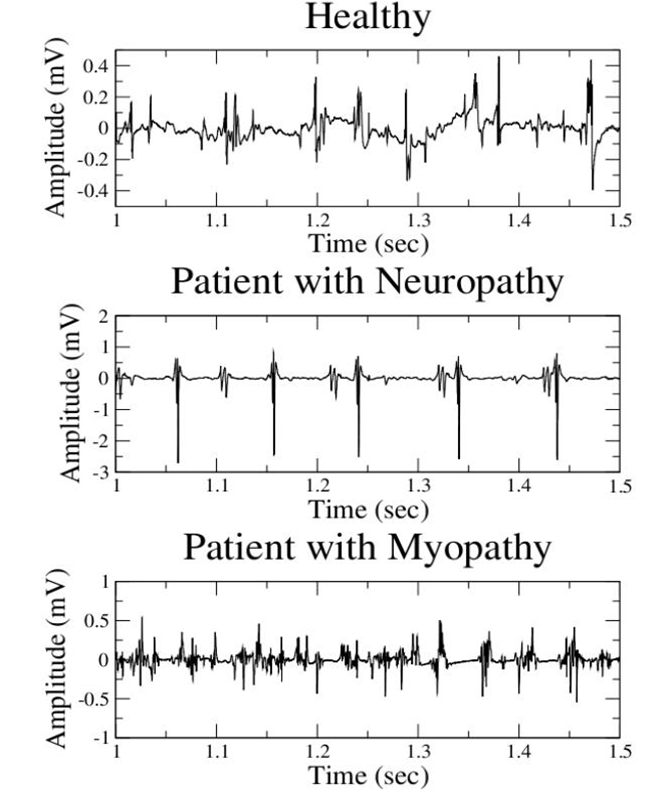
\includegraphics[width=\textwidth]{./img/disorders.png}
					\end{center}
				\end{figure}
				
			\column{.5\textwidth}
				\begin{figure}
					Controle de Próteses Mioelétricas
					\begin{center}
						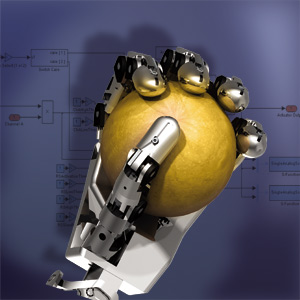
\includegraphics[width=\textwidth]{./img/prosthesis.jpg}
					\end{center}
				\end{figure}
		\end{columns}
	\end{frame}
	
%	\subsection[NinaPro]{Base de Dados NinaPro}
	
	\begin{frame}
		\frametitle{NinaPro}
		\framesubtitle{\emph{Non-Invasive Adaptive Hand Prosthetics} - IDIAP \emph{Research Institute 2012}}
		\begin{columns}[c]
			\column{\textwidth}
				\begin{figure}
					Posicionamento de Eletrodos \\ 12 Canais
					\begin{center}
						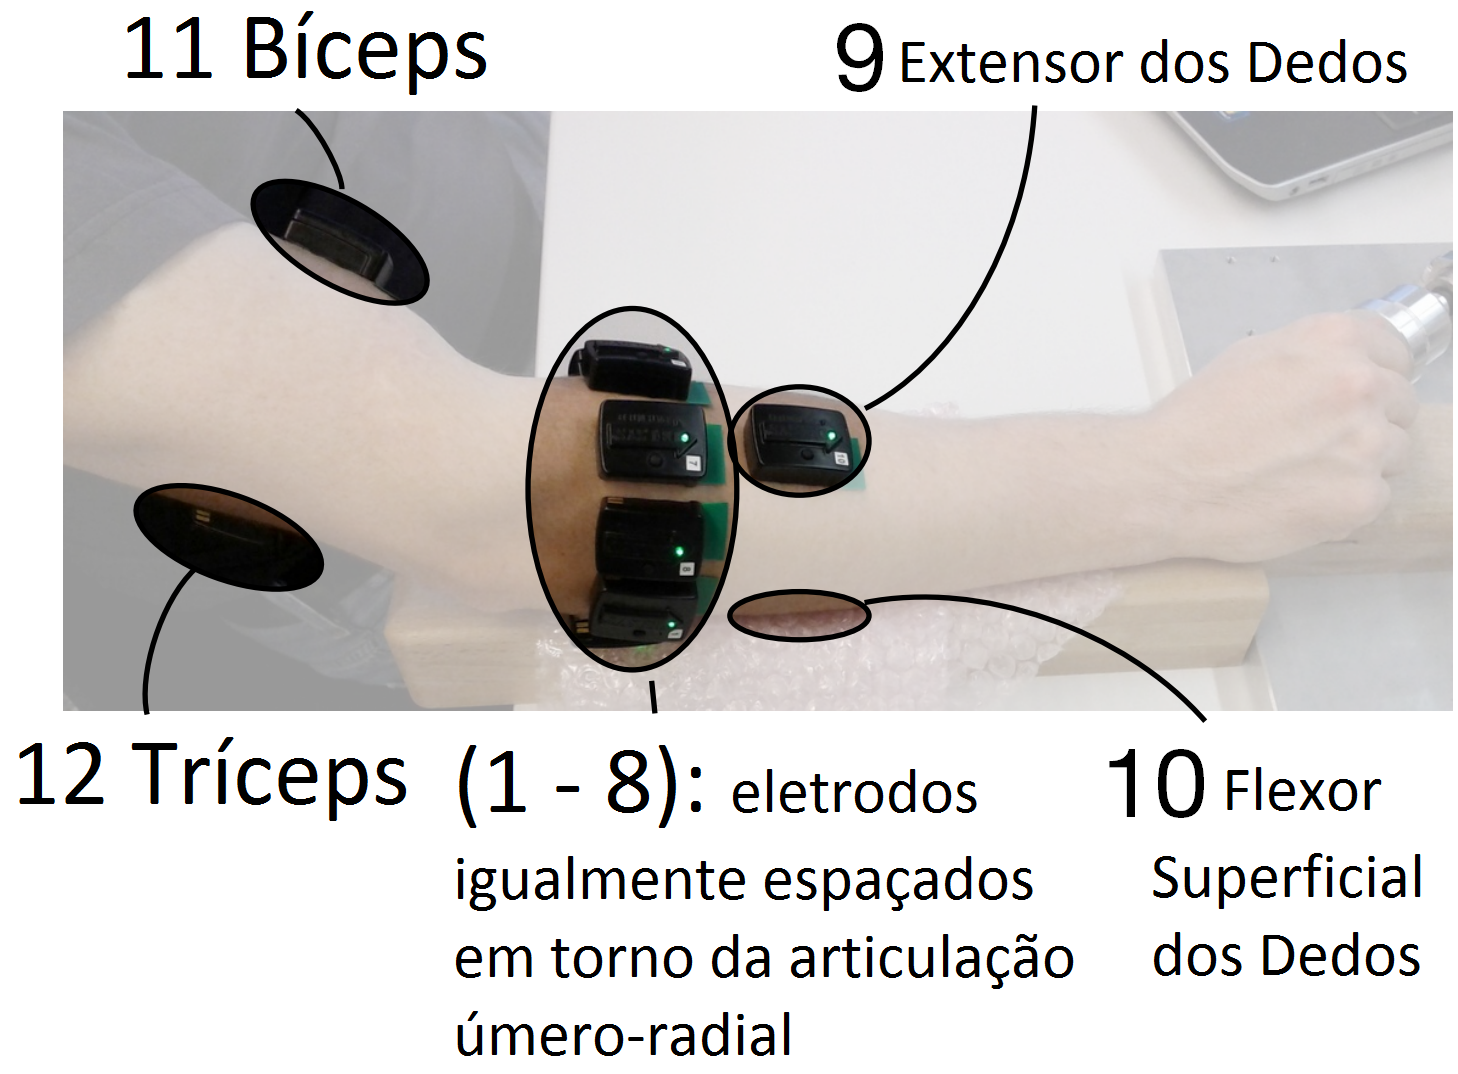
\includegraphics[width=0.8\textwidth]{./img/eletrodos.png}
					\end{center}
				\end{figure}
		\end{columns}
	\end{frame}
	
	\begin{frame}
		\frametitle{Rotina de Aquisição}
		\framesubtitle{Voluntários replicam movimentos apresentados em vídeo}
		\begin{figure}
			Repetição de Movimentos de Vídeo
			\begin{center}
				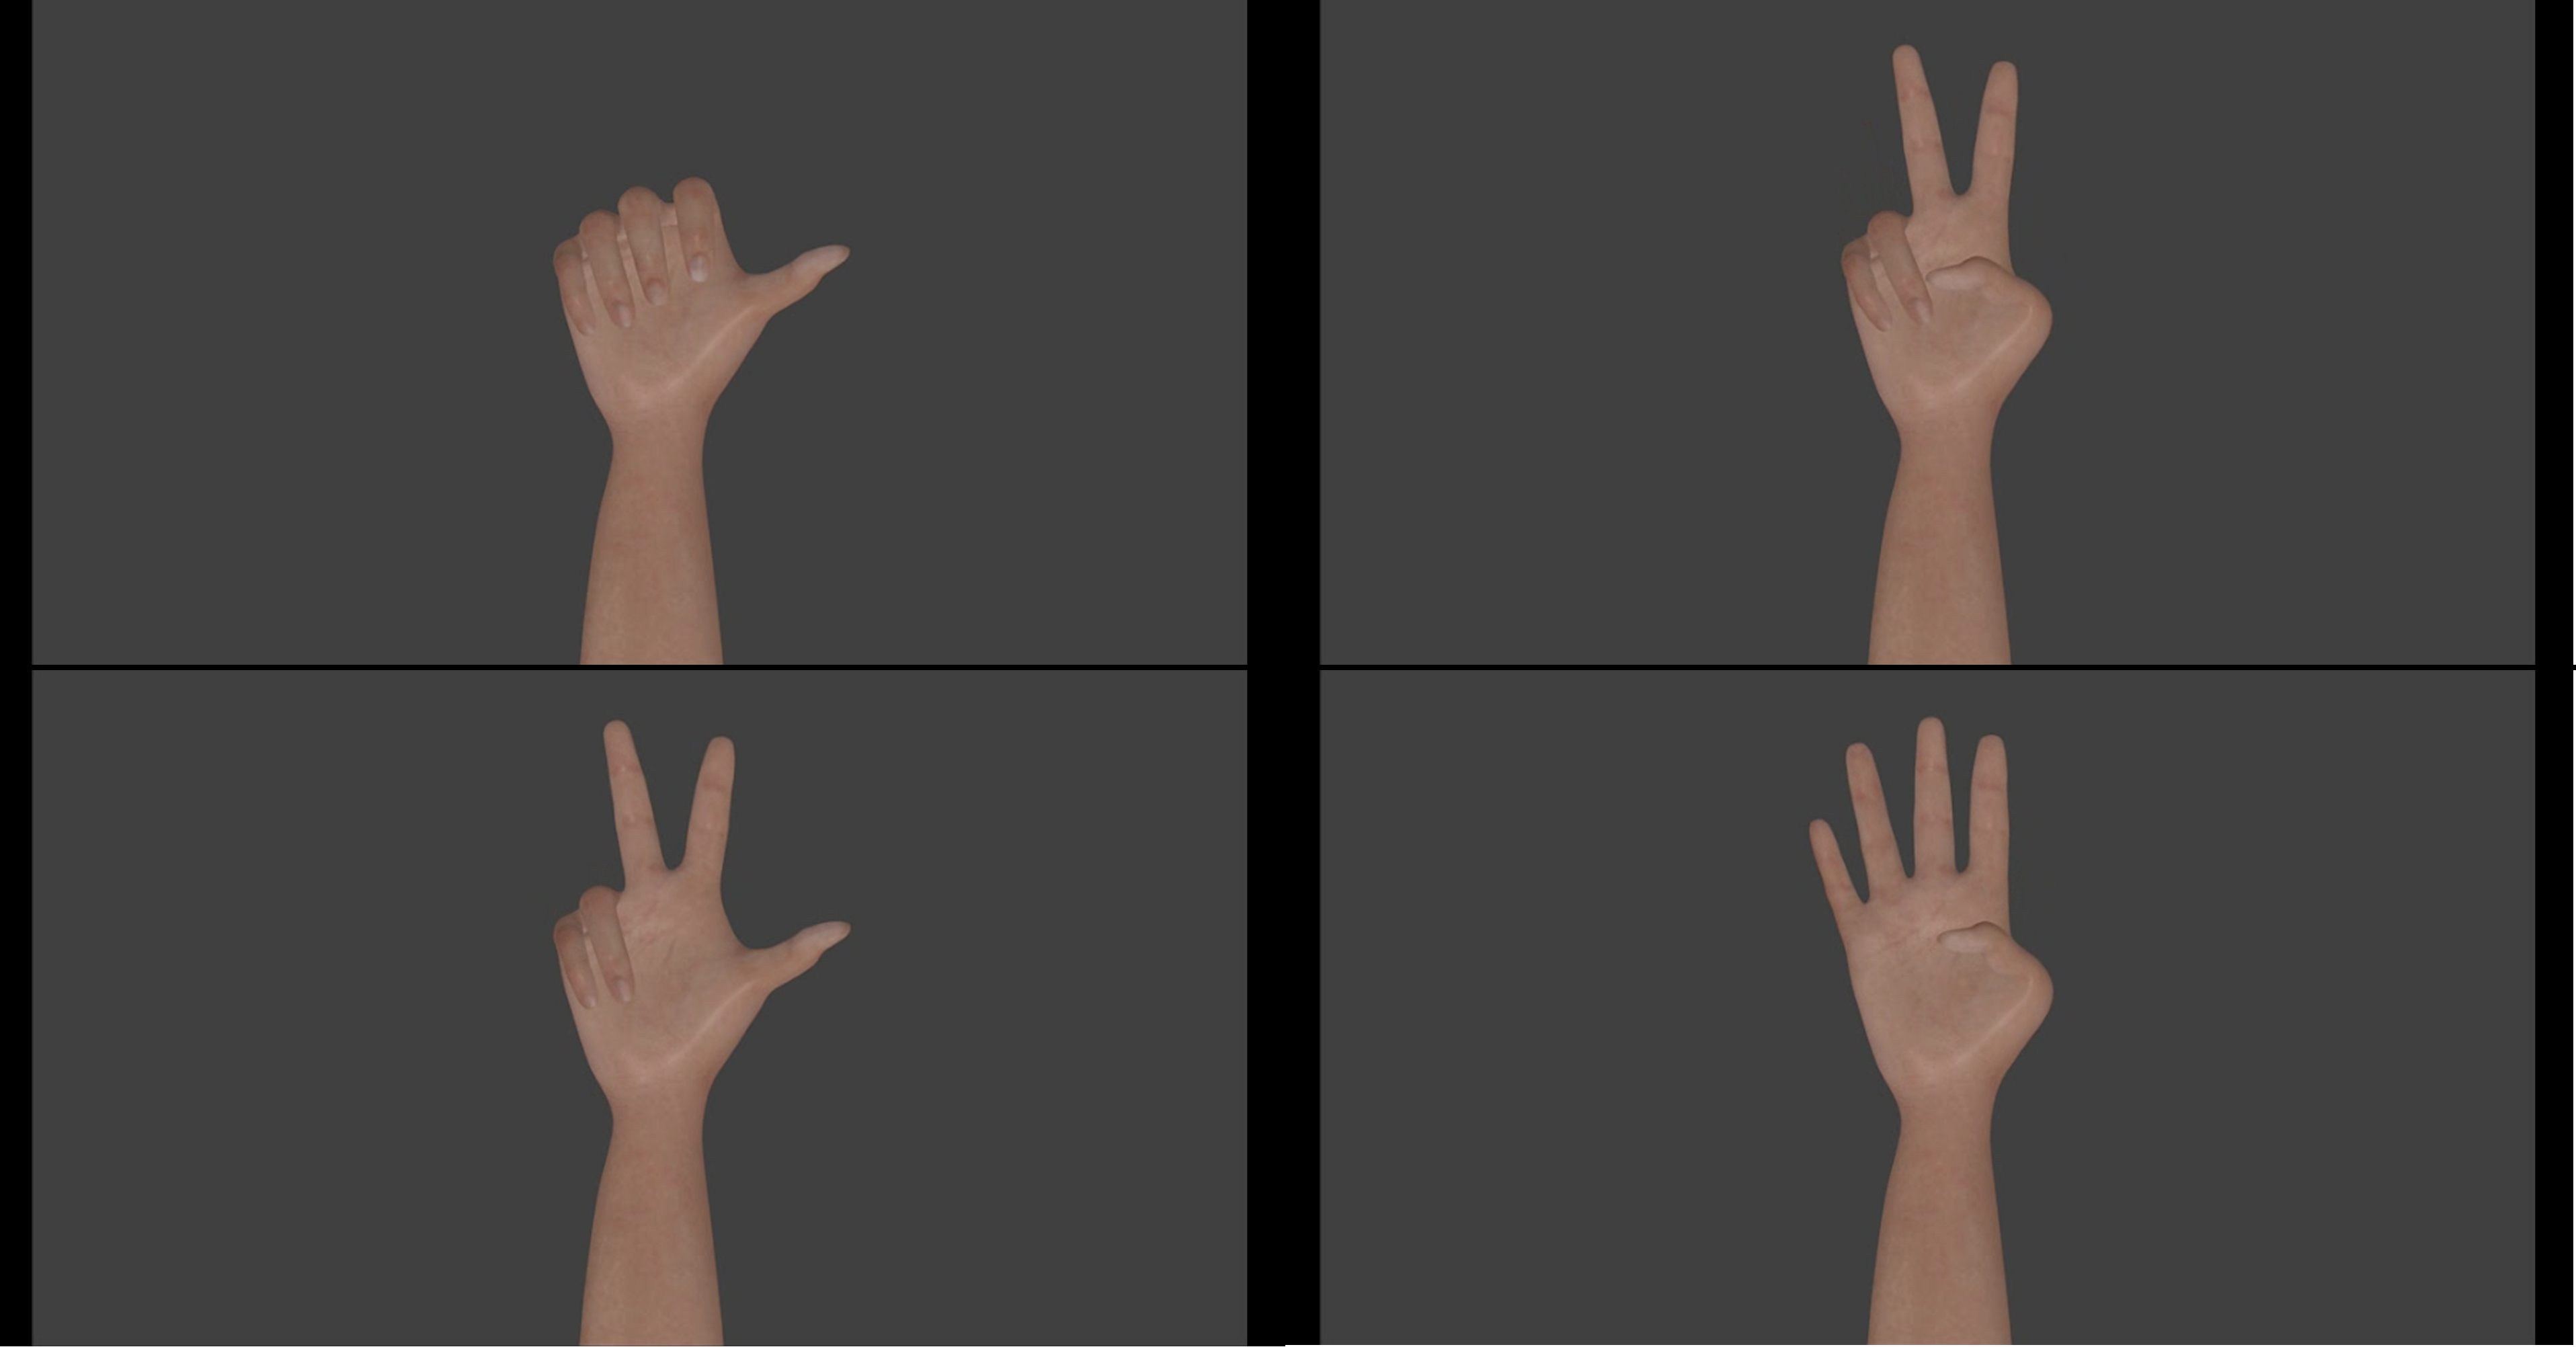
\includegraphics[width=0.7\textwidth]{./img/scenes.png}
			\end{center}
		\end{figure}
		\begin{alertblock}{17 diferentes movimentos de mão e punho}
			6 repetições por movimento \\
			5 segundos de duração por repetição \\
			3 segundos de pausa entre repetições
		\end{alertblock}
	\end{frame}
	
	\begin{frame}
		\frametitle{Classificação de Movimentos}
		%\framesubtitle{A classificação do movimento realizado pode ser utilizado}
		
		\begin{exampleblock}{Classificação de Movimentos}
			O uso de um método classificador (e.g. RNA) pode identificar o movimento realizado pelo voluntário.
		\end{exampleblock}
		
		\begin{figure}
			\begin{center}
				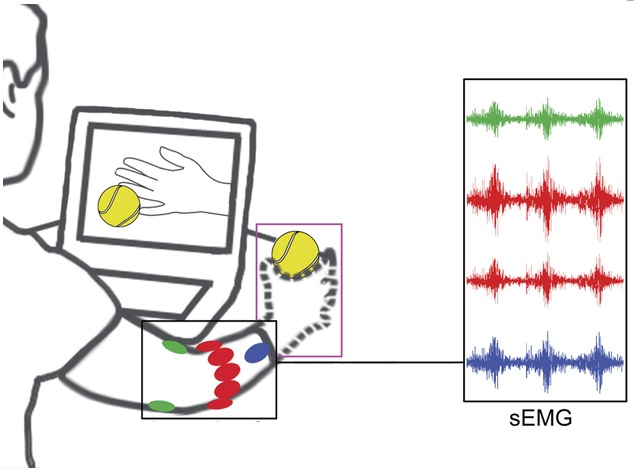
\includegraphics[width=0.9\textwidth]{./img/classificationExample.jpg}
			\end{center}
		\end{figure}
		
	\end{frame}
	
	\begin{frame}
		\frametitle{Objetivos do Trabalho}
		
		\begin{alertblock}{Etapas Necessárias para a Classificação de Movimentos}
		\begin{itemize}
			\item Segmentação do Sinal em Trechos de Interesse
			\item Extração de Características dos Segmentos
			\item Treinamento de RNA
		\end{itemize}
		\end{alertblock}
		
		\begin{block}{Objetivos deste Trabalho}
			Implementação de métodos de segmentação propostos e avaliação comparativa entre métodos quando utilizados para classificação de movimentos com uso de RNA.
		\end{block}
		
		\begin{columns}[c]
		
			\column{.45\textwidth}
				\begin{exampleblock}{Características Extraídas}
					\begin{itemize}
						\item RMS
						\item Variância
						\item Frequência Mediana
					\end{itemize}
				\end{exampleblock}
				
			\column{.45\textwidth}
				\begin{exampleblock}{Bases de Dados Utilizadas}
					Ninapro: 40 voluntários\\
					IEE: 10 voluntários
				\end{exampleblock}
		
		\end{columns}
	\end{frame}

	\section[Métodos Propostos]{Métodos Propostos}
	
	\subsection[MTD1]{MTD1}
	\begin{frame}
		\frametitle{MTD1}
		\framesubtitle{Método iterativo utilizando threshold de amplitudes, segmentos de comprimento constante}
		
		Baseado em Chauvet et al. (2001)
		
		\begin{block}{MTD1}
			EXPLICAÇÕES DO MÉTODO
		\end{block}
		
		EQUAÇÕES DO MÉTODO E IMAGEM ILUTRATIVA
		
	\end{frame}
	
%	\begin{frame}
%			IMAGEM ILUSTRANDO O MTD1
%	\end{frame}
	
	\subsection[MTD2]{MTD2}
	\begin{frame}
		\frametitle{MTD2}
		\framesubtitle{Método não-iterativo utilizando threshold de amplitudes, segmentos de comprimento constante}
		
		Baseado em Katsis et al. (2006)
		
		\begin{block}{MTD2}
			EXPLICAÇÕES DO MÉTODO
		\end{block}
		
		EQUAÇÕES DO MÉTODO E IMAGEM ILUTRATIVA
		
	\end{frame}
	
	\subsection[MTD3]{MTD3}
	\begin{frame}
		\frametitle{MTD3}
		\framesubtitle{Método com janela deslizante utilizando variação total, segmentos de comprimento variável}
		
		Baseado em Gut e Moschytz (2000)
		
		\begin{block}{MTD3}
			EXPLICAÇÕES DO MÉTODO
		\end{block}
		
		EQUAÇÕES DO MÉTODO E IMAGEM ILUTRATIVA
		
	\end{frame}
	
	\subsection[MTD4]{MTD4}
	\begin{frame}
		\frametitle{MTD4}
		\framesubtitle{Método com janela deslizante utilizando threshold, segmentos de comprimento variável}
		
		Baseado em Pattichis, Schizas e Middleton (1995)
		
		\begin{block}{MTD4}
			EXPLICAÇÕES DO MÉTODO
		\end{block}
		
		EQUAÇÕES DO MÉTODO E IMAGEM ILUTRATIVA
		
	\end{frame}

	\section[Implementação]{Detalhes de Implementação dos Métodos e RNA}
	
	\begin{frame}
		\frametitle{Preprocessamento}
		\framesubtitle{Retificação e Normalização}
		\begin{figure}
			\begin{center}
				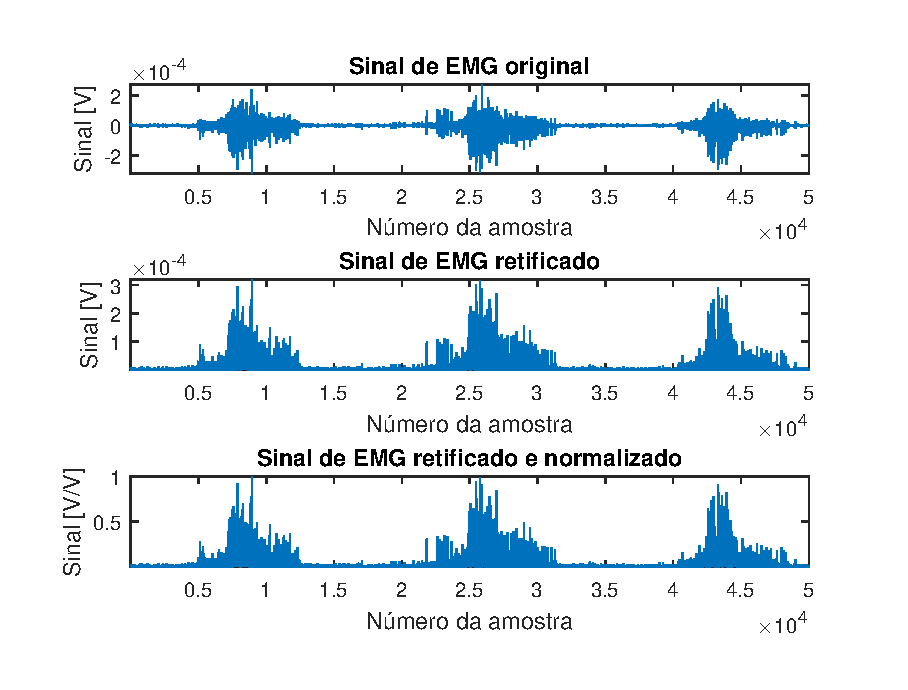
\includegraphics[width=\textwidth]{./img/prettyRaw.eps}
			\end{center}
		\end{figure}
	\end{frame}
	
	\begin{frame}
		\frametitle{DBSCAN}
		\framesubtitle{Agrupamento de segmentos obtidos nos 12 canais de aquisição}
		\begin{exampleblock}{Agrupamento por DBSCAN}
			A partir da densidade de posições de segmentos obtidas nos diferentes canais, identifica-se os segmentos referentes a um mesmo trecho de interesse. Segmentação final é realizada nas posições médias de grupos de segmentos.
		\end{exampleblock}
		IMAGEM ILUSTRANDO USO DE DBSCAN
	\end{frame}
	
	\begin{frame}
		\frametitle{RNA}
		\framesubtitle{Treinamento e simulação de redes neurais artificiais}
		\begin{alertblock}{Divisão de Grupos para Treino, Validação e Teste}
			Para $N_\zeta$ segmentos obtidos referentes à classe de movimento $\zeta$ \\
			\begin{itemize}
				\item Grupo de Treino: primeiros $N_\zeta-2$ segmentos
				\item Grupo de Validação: segmento de índice $N_\zeta-1$
				\item Grupo de Teste: $N_\zeta$-ésimo segmento
			\end{itemize}
		\end{alertblock}
		\begin{figure}
			\begin{center}
				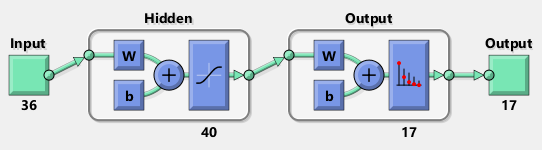
\includegraphics[width=\textwidth]{./img/matlabRNA.png}
			\end{center}
		\end{figure}
	\end{frame}

	\section[Resultados]{Resultados}
	\subsection[Testes com Diferentes Combinações de Parâmetros]{Testes com Diferentes Combinações de Parâmetros}
	
	\begin{frame}
		\frametitle{Testes com Diferentes Combinações de Parâmetros}
		\framesubtitle{MTD1 e MTD2}
		\begin{columns}[c]
		
		\column{.5\textwidth}
			\begin{figure}
				\begin{center}
					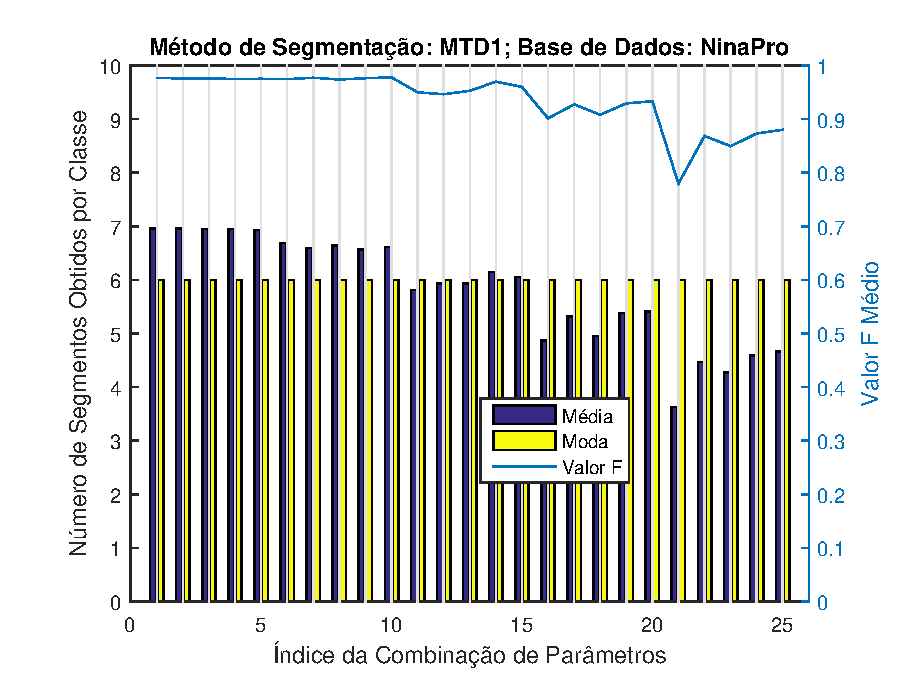
\includegraphics[width=0.8\textwidth]{./img/mtd1_nina.eps}
				\end{center}
			\end{figure}
			\begin{figure}
				\begin{center}
					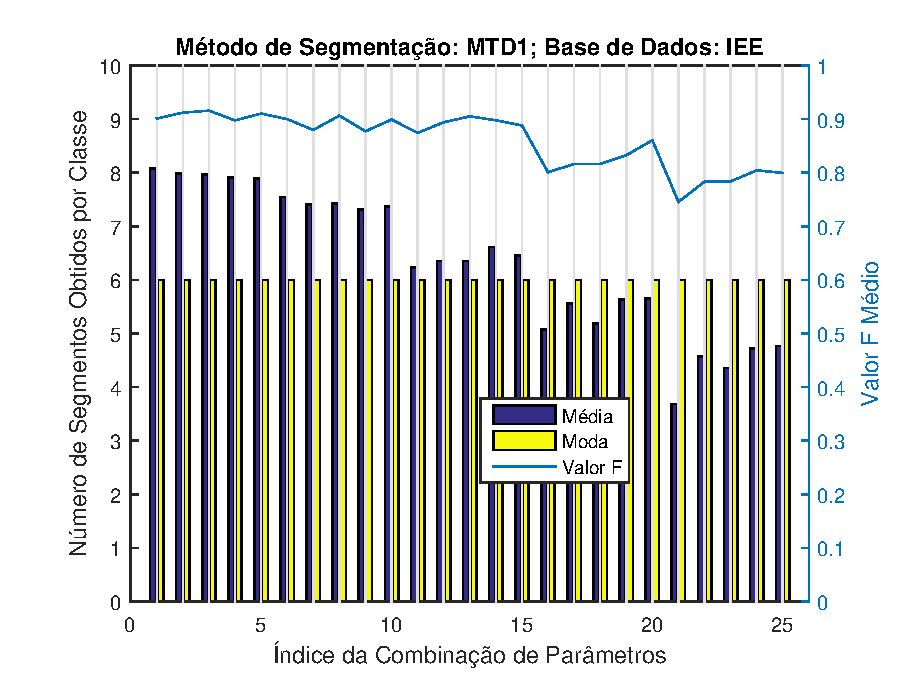
\includegraphics[width=0.8\textwidth]{./img/mtd1_iee.eps}
				\end{center}
			\end{figure}
			
		\column{.5\textwidth}
			\begin{figure}
				\begin{center}
					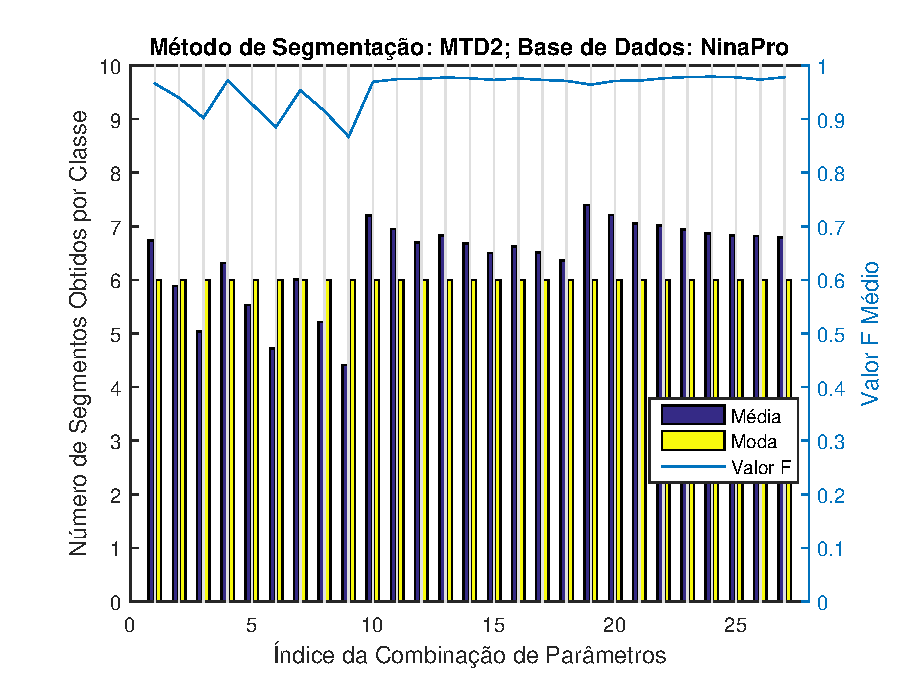
\includegraphics[width=0.8\textwidth]{./img/mtd2_nina.eps}
				\end{center}
			\end{figure}
			\begin{figure}
				\begin{center}
					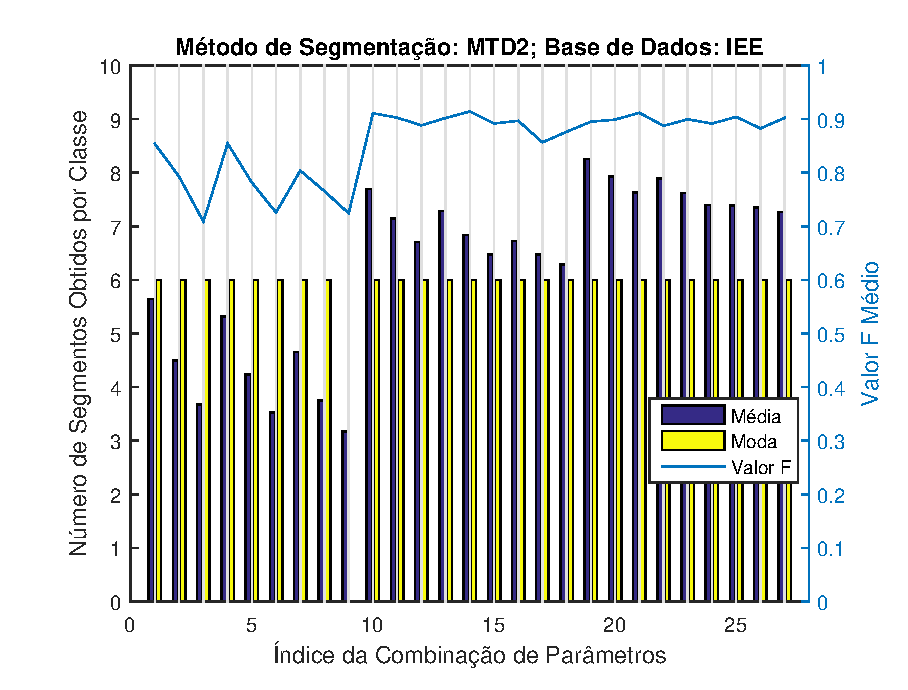
\includegraphics[width=0.8\textwidth]{./img/mtd2_iee.eps}
				\end{center}
			\end{figure}
			
		\end{columns}
	\end{frame}
	
	\begin{frame}
		\frametitle{Testes com Diferentes Combinações de Parâmetros}
		\framesubtitle{MTD3 e MTD4}
		\begin{columns}[c]
		
		\column{.5\textwidth}
			\begin{figure}
				\begin{center}
					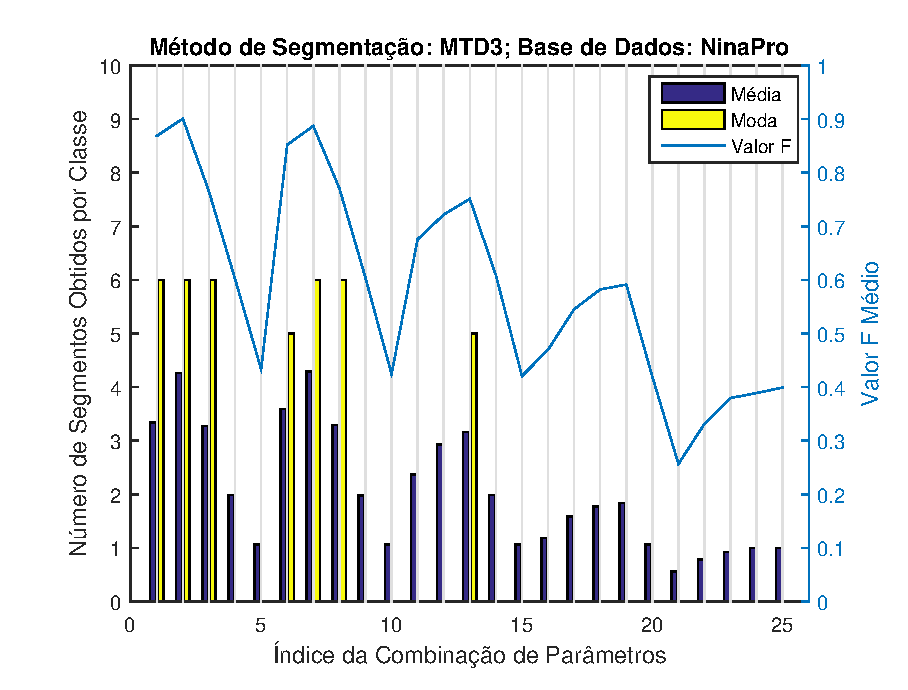
\includegraphics[width=0.8\textwidth]{./img/mtd3_nina.eps}
				\end{center}
			\end{figure}
			\begin{figure}
				\begin{center}
					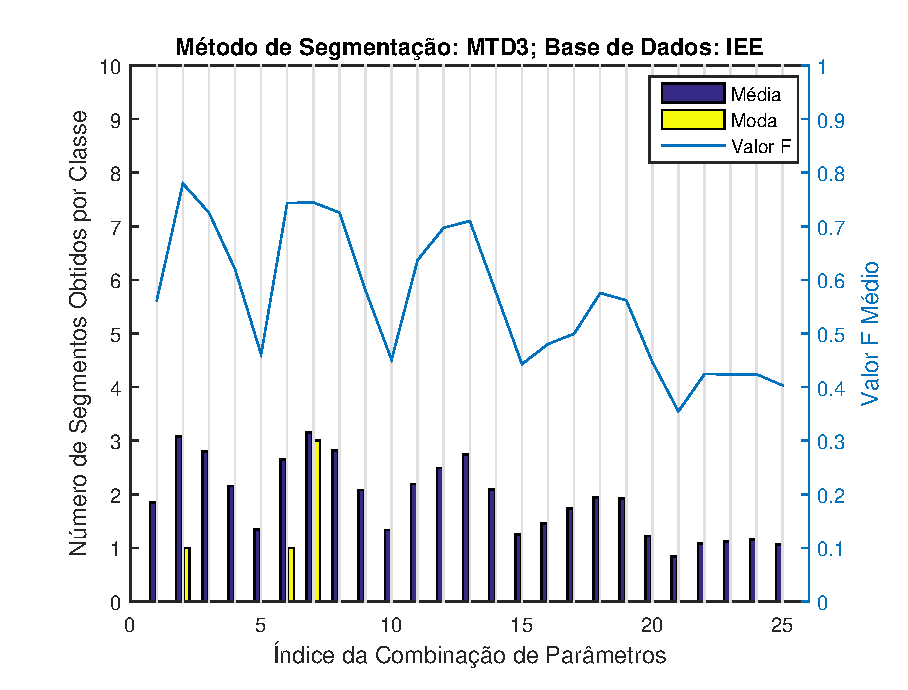
\includegraphics[width=0.8\textwidth]{./img/mtd3_iee.eps}
				\end{center}
			\end{figure}
			
		\column{.5\textwidth}
			\begin{figure}
				\begin{center}
					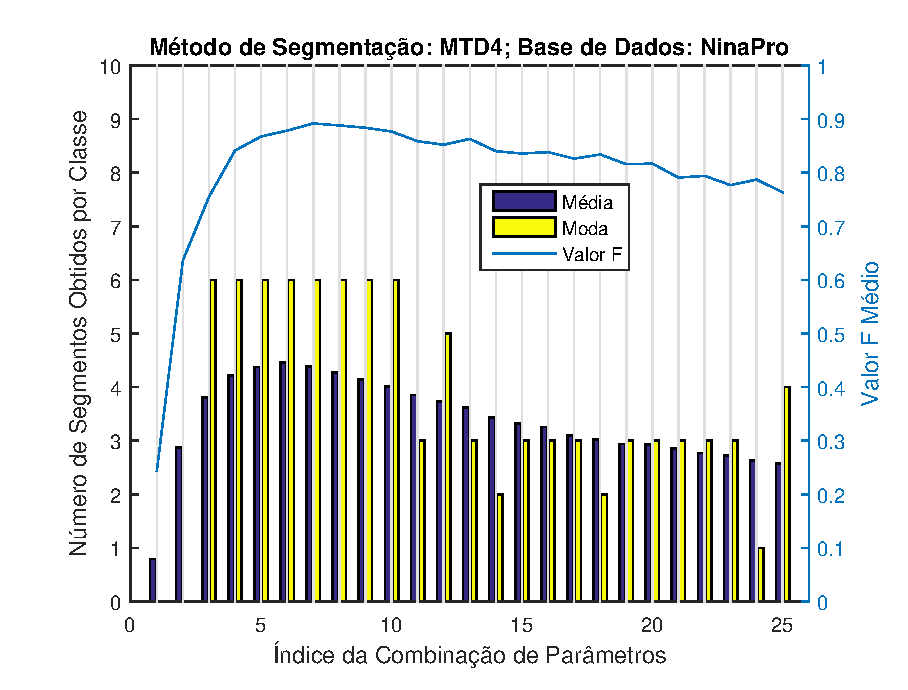
\includegraphics[width=0.8\textwidth]{./img/mtd4_nina.eps}
				\end{center}
			\end{figure}
			\begin{figure}
				\begin{center}
					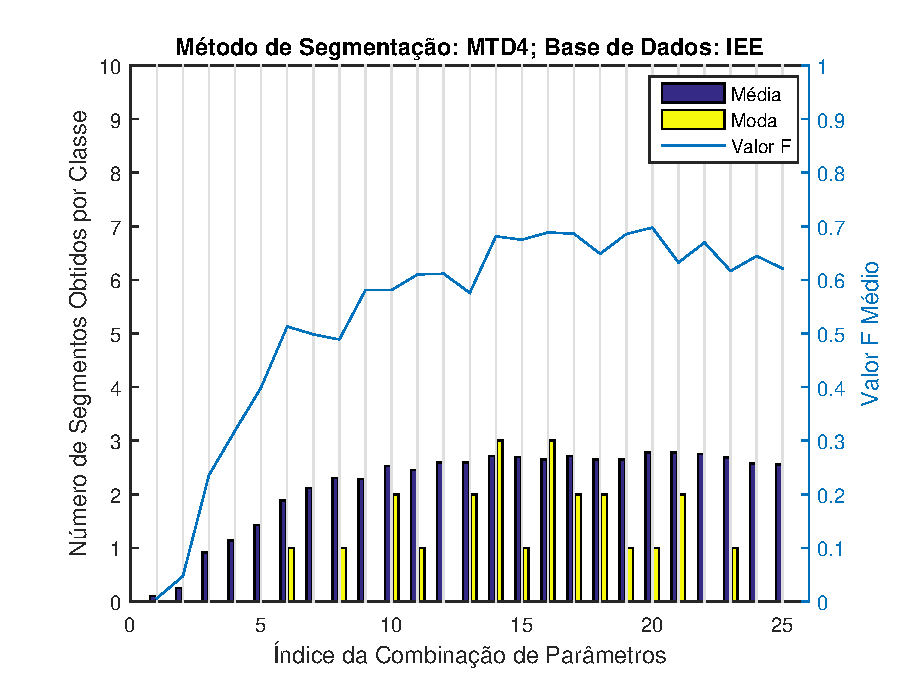
\includegraphics[width=0.8\textwidth]{./img/mtd4_iee.eps}
				\end{center}
			\end{figure}
			
		\end{columns}
	\end{frame}
	
	\subsection[Resultados Utilizando Parâmetros Selecionados]{Resultados Utilizando Parâmetros Selecionados}
	
	\begin{frame}
		\frametitle{Resultados Utilizando Parâmetros Selecionados}
		\framesubtitle{Valor F por Classe de Movimento, Base de Dados NinaPro}
		
		\begin{figure}
			\begin{center}
				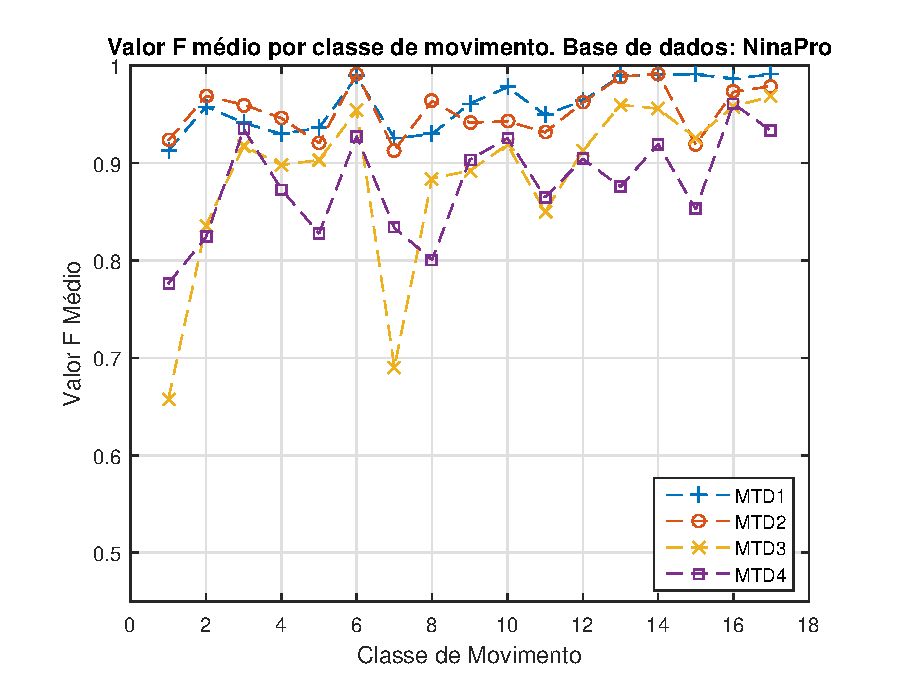
\includegraphics[width=\textwidth]{./img/fvalue_nina.eps}
			\end{center}
		\end{figure}
		
	\end{frame}
	
	\begin{frame}
		\frametitle{Resultados Utilizando Parâmetros Selecionados}
		\framesubtitle{Valor F por Classe de Movimento, Base de Dados IEE}
		
		\begin{figure}
			\begin{center}
				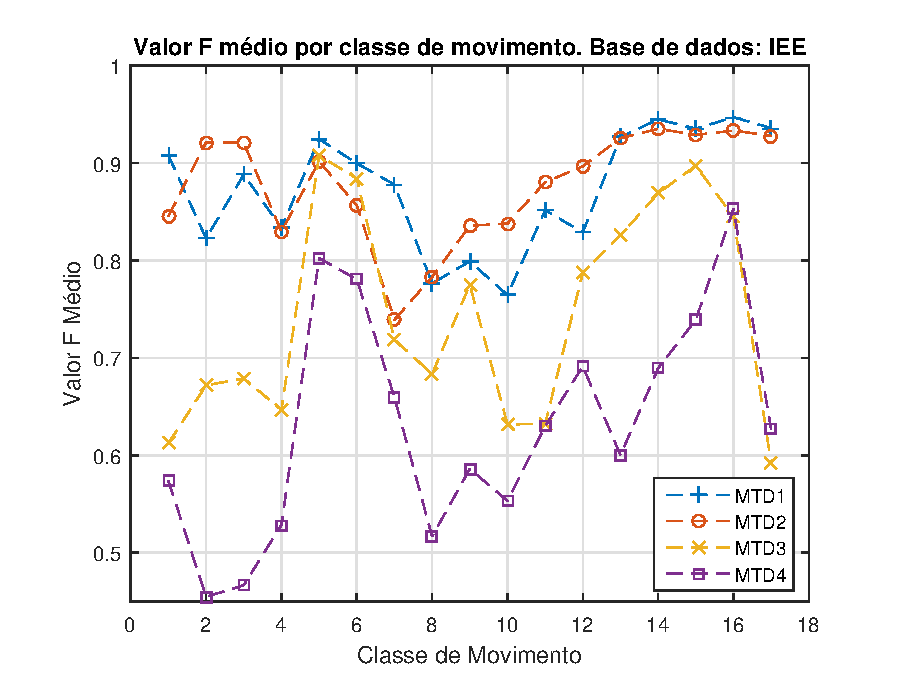
\includegraphics[width=\textwidth]{./img/fvalue_iee.eps}
			\end{center}
		\end{figure}
		
	\end{frame}
	
	\section[Conclusões]{Conclusões}

		\begin{frame}
		\frametitle{Conclusões}
		\framesubtitle{TODO}
		\begin{itemize}
		\item MELHORES E PIORES CLASSIFICAÇÕES OBTIDAS COM CADA MÉTODO
		\item COMPARAÇÕES ENTRE MÉTODOS
		\end{itemize}
		\end{frame}

\end{document}